
\noindent Schema:

\begin{figure}[H]
  \begin{center}
  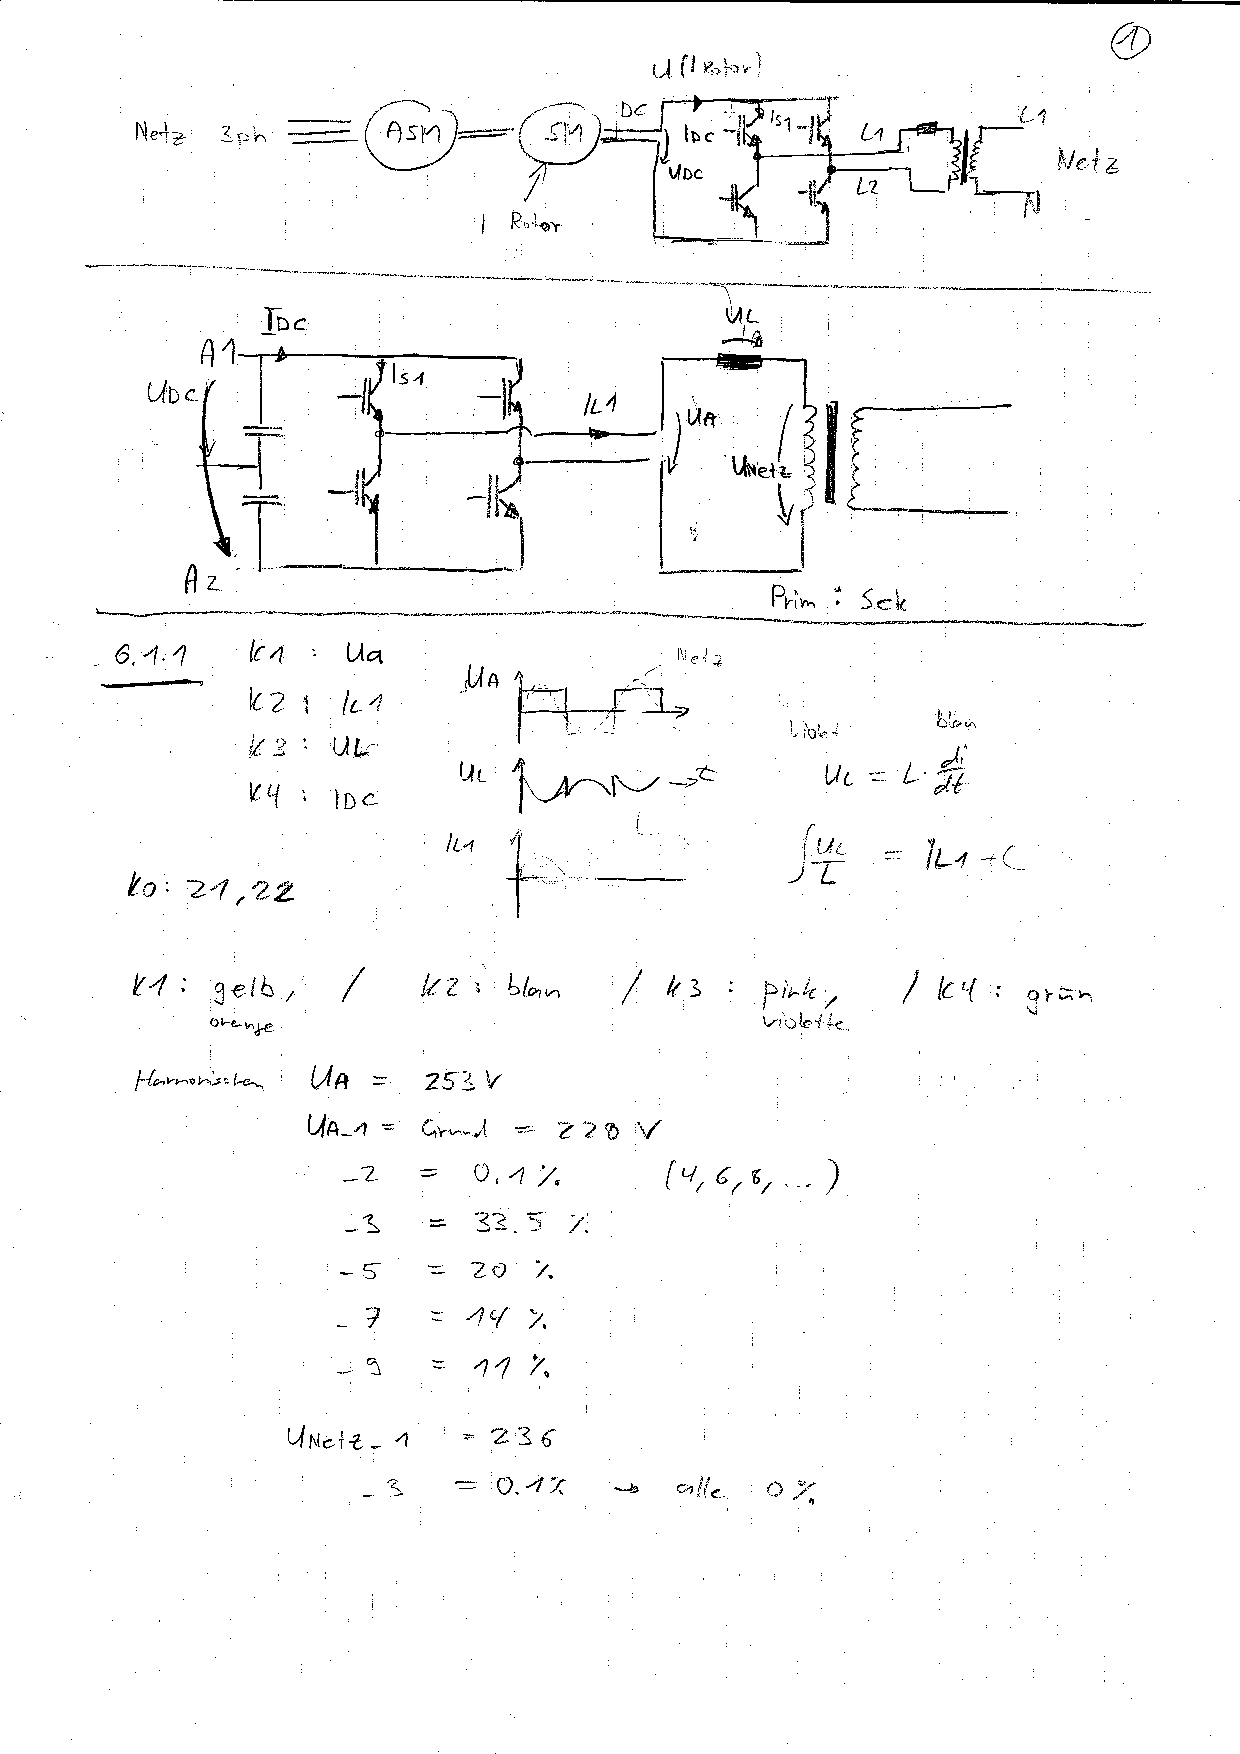
\includegraphics[width=1\textwidth, trim={1cm 19.38cm 1cm 5cm},clip]{notes/scan1.pdf}
  \caption{Schema}
  \label{fig:schema}
  \end{center}
\end{figure}


Kanalbelegung beim KO:


\begin{table}[h]
  \centering
  \begin{tabular}{ l | l | l }
    \hline 
    Channel & Farbe & Bezeichnung \\
    \hline \hline
    1 & gelb / orange &  $U_A$ \\
    \hline
    2 & hellblau & $I_{L1}$ , da Einphasig\\  
    \hline 
    3 & pink / violette & $U_{L}$ \\  
    \hline
    4 & grün & $I_{DC}$ \\  
    \hline
  \end{tabular}
  \caption{Kanalbelegung}
  \label{tab:Kanalbelegung}
\end{table}




\clearpage